% cap4.tex

\chapter{Análisis de Resultados}
\label{c4} % la etiqueta para referencias
En el presente capítulo se exponen los resultados obtenidos de la ejecución del modelo de equilibrio bajo condiciones de inatención conductual. El objetivo es analizar cómo la capacidad de procesamiento de información del planificador impacta en la transición energética de Chile para el período 2020--2030. Para esto, el capítulo se estructura en cuatro partes principales: primero, se calibra el nivel de atención ($m$) para ver qué nivel de atención es el que tiene Chile de acuerdo a la matriz energética real del 2024 (según los parámetros que usa el modelo); segundo, se obtiene el valor de  $\sigma_{\varepsilon}$ a través de la calibración explicada en la sección anterior y su impacto en los costos; tercero, se evalúa cómo varían el presupuesto óptimo, los precios y la inversión según el grado de atención; y finalmente, se detalla la evolución tecnológica de la matriz y el cumplimiento de las metas de emisiones hacia el año 2030.

Como base para el desarrollo de este capítulo, se resumen los parámetros encontrados en el Capítulo \ref{c3} en el Cuadro \ref{tab:resumen_parametros}:
\begin{table}[H]
\centering
\caption{Resumen de parámetros base para la simulación}
\label{tab:resumen_parametros}
\renewcommand{\arraystretch}{1.2}
\setlength{\tabcolsep}{10pt}
\begin{tabular}{l c l}
\toprule
\textbf{Parámetro} & \textbf{Valor} & \textbf{Unidad} \\
\midrule
$CAP_s$ & 264,20 & MtCO$_2$e \\
$CAP_d$ & 311,00 & MtCO$_2$e \\
$\sigma_{CAP}$ & 61,86& MtCO$_2$e \\
$\kappa$ & 64,40 & USD/tCO$_2$e \\
\bottomrule
\end{tabular}

\footnotesize{Fuente: Elaboración propia.}
\end{table}

\section{\boldmath Calibración de $\sigma_\varepsilon$ en la producción energética y resultados para Chile}
La diferencia absoluta al comparar la matriz energética real con la del modelo para el año 2024 y el escenario $\omega=5$, se muestra en el Cuadro \ref{tab:top10_distancia_mix} ordenada de menor a mayor distancia. 

\begin{table}[H]
\centering
\small
\caption{Distancia absoluta entre el mix modelado y el observado para el 2024 (Escenario 5)}
\label{tab:top10_distancia_mix}
\renewcommand{\arraystretch}{1.1}
\setlength{\tabcolsep}{6pt}
\begin{tabular}{c c c}
\toprule
\textbf{$\sigma_{\varepsilon}$ (MtCO$_2$e)} & \textbf{$m$} & \textbf{Distancia absoluta} \\
\midrule
$\infty$ & 0,0 & 0,2727 \\
185,58 & 0,1 & 0,2758 \\
123,72 & 0,2 & 0,2788 \\
94,49  & 0,3 & 0,2818 \\
75,76  & 0,4 & 0,2849 \\
61,86  & 0,5 & 0,2879 \\
50,51  & 0,6 & 0,2909 \\
40,50  & 0,7 & 0,2940 \\
30,93  & 0,8 & 0,2970 \\
20,62  & 0,9 & 0,2998 \\
0,00   & 1,0 & 0,3026 \\
\bottomrule
\end{tabular}

\vspace{0.15cm}
\footnotesize{Fuente: Elaboración propia.}
\end{table}
                  
Como puede observarse en el Cuadro \ref{tab:top10_distancia_mix}, el menor valor de la distancia absoluta se obtiene para un nivel de error extremadamente alto, lo cual hace que la atención sea cero, lo que sugiere que el sistema eléctrico chileno observado es más consistente con un comportamiento de atención mínima por parte del planificador, guiándose completamente por experiencias pasadas o conocimiento predeterminado para la elección del presupuesto ($CAP_d$). \medskip

Para valores moderadamente bajos de atención respecto al ruido, en particular $m = 0{,}1$, $m = 0{,}2$ y $m = 0{,}3$, la distancia respecto del mix real se mantiene similar y cercana al mínimo de 0,2727, lo que indica que dichos niveles continúan ofreciendo un ajuste razonable de la composición tecnológica observada. A medida que el error disminuye, la distancia aumenta de manera progresiva, reflejando una mayor desviación entre la matriz energética simulada y la real. \medskip

Para los análisis que vendrán más adelante, se seleccionó el nivel de $\sigma_\varepsilon$ que permite obtener un valor determinado y minimice la distancia absoluta entre los datos reales y simulados; este corresponde a  $\sigma_{\varepsilon} = 186,90$ con una diferencia de 0,2758. Dicho nivel es coherente con un nivel de atención $m=0,1$. 

Con este parámetro, se pueden construir escenarios representativos para el presupuesto real enfrentado por el agente, asumiendo que el error de la señal $\epsilon$ es equivalente a $\sigma_{\varepsilon}$, de esta forma, el presupuesto real ($CAP$) se puede expresar como $CAP = CAP_s \pm \sigma_{\varepsilon}$. Con esto se construye el Cuadro \ref{tab:cap_pos_neg_mm} que muestra los dos valores de $CAP$ obtenidos, donde $CAP+$ representa el $CAP+\sigma_\varepsilon$ y $CAP-$ representa el $CAP-\sigma_\varepsilon$; también se muestra el $\theta^*$ encontrado, la diferencia entre ambos y por último el costo y la utilidad que se extraen al reemplazar los valores correspondientes en la formulación \ref{eq:utilidadv}.

\begin{table}[H]
\centering
\caption{Comportamiento de la función de utilidad bajo escenarios $CAP^{+}$ y $CAP^{-}$ para $m=0,1$}
\label{tab:cap_pos_neg_mm}
\small
\renewcommand{\arraystretch}{1.15}
\setlength{\tabcolsep}{8pt}
\begin{tabular}{l c c c c c}
\toprule
\textbf{Escenario} &
\textbf{CAP} &
$\boldsymbol{\theta^*}$ &
$\boldsymbol{\theta^* - CAP}$ &
\textbf{Costo} &
\textbf{Utilidad} \\
 & (MtCO$_2$) & (MtCO$_2$) & (MtCO$_2$) & (M USD) & (M USD) \\
\midrule
$CAP^{+}$ &
449,78 &
306,33 &
-143,45 &
662.589.589.804,07 &
-662.589.533.175,84 \\

$CAP^{-}$ &
78,62 &
306,33 &
227,71 &
1.669.659.335.377,53 &
-1.669.659.278.749,30 \\
\bottomrule
\end{tabular}

\vspace{0.15cm}
\footnotesize{\textit{Fuente: Elaboración propia.}}
\end{table}
Se observa que la diferencia entre la meta fijada ($\theta$) y el presupuesto real ($CAP$) genera una desviación que, al elevarse al cuadrado en el término de penalización, resulta en una utilidad negativa. El valor de esta pérdida es más acentuado en el escenario $CAP^{-}$ debido a que la brecha respecto a la meta óptima es mayor que en el escenario opuesto.

\section{Resultados para distintos niveles de atención.}
El Cuadro \ref{tab:resultados_agregados_m} presenta los resultados del presupuesto de emisiones óptimas ($\theta^*$), el precio de venta $\pi^a$, las emisiones y la capacidad instalada (GW), para distintos niveles de atención. A partir de estos resultados se observa que, a medida que el nivel de atención aumenta y el presupuesto de emisiones se vuelve más restrictivo, el precio de los permisos de emisión tiende a incrementarse. Por otra parte, dado que el sistema debe mantener un nivel de producción constante, la reducción en las emisiones se logra principalmente mediante un cambio en la matriz tecnológica sustituyendo tecnologías fósiles por tecnologías limpias. Estas últimas presentan factores de planta más bajos (Véase el Anexo \ref{tab:epsilon}), por lo que para producir la misma cantidad de energía, es necesario instalar una mayor capacidad. Esto explica que bajo escenarios con mayor atención y menor presupuesto de emisiones, se observe un aumento en la inversión total del sistema en términos de capacidad instalada.

\begin{table}[H]
\centering
\caption{Resultados agregados del modelo bajo distintos niveles de atención}
\label{tab:resultados_agregados_m}
\renewcommand{\arraystretch}{1.2}
\setlength{\tabcolsep}{8pt}
\small
\begin{tabular}{c c c c c}
\toprule
\textbf{$\boldsymbol{m}$} &
\makecell{\textbf{$\boldsymbol{\theta^*}$} \\ \textbf{(tCO$_2$e)}} &
\makecell{\textbf{$\boldsymbol{\pi^a}$} \\ \textbf{(USD/tCO$_2$e)}} &
\makecell{\textbf{Emisiones} \\ \textbf{totales (MtCO$_2$e)}} &
\makecell{\textbf{Capacidad} \\ \textbf{Instalada (GW)}} \\
\midrule
0,0 & 311\,013\,380,4 & 183,319 & 311,013 & 20,873 \\
0,1 & 306\,332\,042,7 & 184,859 & 306,332 & 21,120 \\
0,2 & 301\,650\,704,9 & 186,400 & 301,651 & 21,366 \\
0,3 & 296\,969\,367,2 & 187,940 & 296,969 & 21,614 \\
0,4 & 292\,288\,029,5 & 189,480 & 292,288 & 21,861 \\
0,5 & 287\,606\,691,7 & 191,021 & 287,607 & 22,108 \\
0,6 & 282\,925\,354,0 & 192,561 & 282,925 & 22,356 \\
0,7 & 278\,244\,016,3 & 194,101 & 278,244 & 22,603 \\
0,8 & 273\,562\,678,5 & 195,681 & 273,563 & 22,853 \\
0,9 & 268\,881\,340,8 & 197,216 & 268,881 & 23,103 \\
1,0 & 264\,200\,003,1 & 198,751 & 264,200 & 23,353 \\
\bottomrule
\end{tabular}

\vspace{0.1cm}
\footnotesize{\textit{Fuente: Elaboración propia.}}

\end{table}

De la misma manera que se construyó el Cuadro \ref{tab:cap_pos_neg_mm} se construyen los Cuadros \ref{tab:resultados_m} y  \ref{tab:resultados_m_2}, pero para todos los niveles de atención con el fin de facilitar la comparación.

% \begin{table}[H]
% \centering
% \caption{Resultados del modelo bajo escenarios $CAP^{+}$ y $CAP^{-}$ para distintos niveles de atención}
% \label{tab:cap_pm_por_m}
% \footnotesize
% \renewcommand{\arraystretch}{1.15}
% \setlength{\tabcolsep}{6pt}
% \begin{tabular}{c c c c c c c c c c}
% \toprule
% \multicolumn{2}{c}{} &
% \multicolumn{4}{c}{\textbf{Escenario $CAP^{+}$}} &
% \multicolumn{4}{c}{\textbf{Escenario $CAP^{-}$}} \\
% \cmidrule(lr){3-6} \cmidrule(lr){7-10}
% \textbf{$m$} &
% $\boldsymbol{\sigma_{\epsilon}}$ &
% \textbf{$CAP$} &
% $\boldsymbol{\theta - CAP}$ &
% \textbf{Costo} &
% \textbf{Utilidad} &
% \textbf{$CAP$} &
% $\boldsymbol{\theta - CAP}$ &
% \textbf{Costo} &
% \textbf{Utilidad} \\
%  & (MtCO$_2$e) & (MtCO$_2$e) & (MtCO$_2$e) & (MM USD) & (MM USD) & (MtCO$_2$e) & (MtCO$_2$e) & (MM USD) & (MM USD) \\
% \midrule
% 0,0 & N/A & N/A & N/A & N/A & N/A & N/A & N/A & N/A & N/A \\

% 0,1 & 186,90 & 451,10 & $-144,77$ & 674,87 & $-674,87$ & 77,30 & 229,04 & 1.689,12 & $-2.363,99$ \\
% 0,2 & 124,60 & 388,80 & $-87,15$  & 244,57 & $-244,57$ & 139,60 & 162,05 & 845,61 & $-1.090,18$ \\
% 0,3 & 95,17  & 359,37 & $-62,40$  & 125,37 & $-125,37$ & 169,03 & 127,94 & 527,04 & $-652,40$ \\
% 0,4 & 76,30  & 340,50 & $-48,21$  & 74,85  & $-74,85$  & 187,90 & 104,39 & 350,90 & $-425,75$ \\
% 0,5 & 62,30  & 326,50 & $-38,89$  & 48,71  & $-48,71$  & 201,90 & 85,71  & 236,54 & $-285,25$ \\
% 0,6 & 50,87  & 315,07 & $-32,14$  & 33,27  & $-33,27$  & 213,33 & 69,59  & 155,96 & $-189,22$ \\
% 0,7 & 40,79  & 304,99 & $-26,74$  & 23,03  & $-23,03$  & 223,41 & 54,83  & 96,80  & $-119,83$ \\
% 0,8 & 31,15  & 295,35 & $-21,79$  & 15,29  & $-15,29$  & 233,05 & 40,51  & 52,85  & $-68,14$ \\
% 0,9 & 20,77  & 284,97 & $-16,09$  & 8,33   & $-8,33$   & 243,43 & 25,45  & 20,85  & $-29,19$ \\
% 1,0 & 0,00   & 264,20 & 2,44       & 0,19   & 52,51     & 264,20 & 3,76   & 0,45   & 52,51 \\
% \bottomrule
% \end{tabular}

% \vspace{0.2cm}
% \footnotesize{\textit{Nota: Costos y utilidades expresados en miles de millones de USD (MM USD). Fuente: Elaboración propia.}}
% \end{table}

\begin{table}[H]
\centering
\small
\caption{Resultados del modelo para distintos niveles de atención $m$ (Caso $CAP+$)}
\label{tab:resultados_m}
\renewcommand{\arraystretch}{1.1}
\setlength{\tabcolsep}{6pt}
\begin{tabular}{ccccc}
\toprule
$m$ & CAP (MtCO$_2$) & $\theta-CAP$ (MtCO$_2$) & Costo (M USD) & Beneficio (M USD) \\
\midrule
0,0 & N/A & N/A & N/A & N/A \\
0,1 & 449,78 & -143,45 & 662.589.589.804,07 & -662.589.533.175,84 \\
0,2 & 387,92 & -86,27 & 239.644.999.121,04 & -239.644.942.893,35 \\
0,3 & 358,69 & -61,72 & 122.674.630.993,48 & -122.674.575.181,06 \\
0,4 & 339,96 & -47,67 & 73.186.603.953,91 & -73.186.548.571,17 \\
0,5 & 326,06 & -38,45 & 47.612.752.798,72 & -47.612.697.859,80 \\
0,6 & 314,71 & -31,78 & 32.527.377.488,24 & -32.527.323.007,85 \\
0,7 & 304,70 & -26,45 & 22.532.072.038,36 & -22.532.018.030,91 \\
0,8 & 295,13 & -21,57 & 14.977.809.285,24 & -14.977.755.754,22 \\
0,9 & 284,82 & -15,94 & 8.180.115.598,42 & -8.180.062.570,72 \\
1,0 & 264,20 & 0,00 & 0,00 & 52.510,01 \\
\bottomrule
\end{tabular}

\vspace{0.3cm}
\footnotesize Fuente: Elaboración propia.

\end{table}

\vspace{0.5cm}

\begin{table}[H]
\centering
\small
\caption{Resultados del modelo para distintos niveles de atención $m$ (Caso $CAP-$)}
\label{tab:resultados_m_2}
\renewcommand{\arraystretch}{1.1}
\setlength{\tabcolsep}{6pt}

\begin{tabular}{ccccc}
\toprule
$m$ & CAP (MtCO$_2$) & $\theta-CAP$ (MtCO$_2$) & Costo (M USD) & Beneficio (M USD) \\
\midrule
-    & N/A   & N/A   & N/A & N/A \\
0,1 & 78,62 & 227,71 & 1.669.659.335.377,53 & -1.669.659.278.749,30 \\
0,2 & 140,48 & 161,17 & 836.427.074.998,41 & -836.427.018.770,71 \\
0,3 & 169,71 & 127,26 & 521.499.495.445,26 & -521.499.439.632,84 \\
0,4 & 188,44 & 103,85 & 347.276.282.042,91 & -347.276.226.660,18 \\
0,5 & 202,34 & 85,27 & 234.107.160.573,50 & -234.107.105.634,59 \\
0,6 & 213,69 & 69,23 & 154.345.018.699,95 & -154.344.964.219,57 \\
0,7 & 223,70 & 54,54 & 95.785.627.884,60 & -95.785.573.877,16 \\
0,8 & 233,27 & 40,29 & 52.276.698.090,68 & -52.276.644.559,66 \\
0,9 & 243,58 & 25,30 & 20.613.082.650,14 & -20.613.029.622,44 \\
1,0 & 264,20 & 0,00 & 0,00 & 52.510,01 \\
\bottomrule
\end{tabular}

\vspace{0.3cm}
\footnotesize Fuente: Elaboración propia.

\end{table}

Se observa que la utilidad del planificador es negativa en casi todos los escenarios analizados, excepto cuando se tiene una atención $m=1$. Aunque el precio de los permisos de emisión es elevado en comparación con el impuesto al carbono vigente en Chile (5 USD/tCO$_2$e), los costos asociados a las emisiones superan los ingresos obtenidos por su venta. En consecuencia, incluso con precios elevados del carbono, la recaudación del mercado de permisos no logra compensar el daño ambiental considerado en el modelo a menos que se tenga atención perfecta. 

\section{Producción Generada en MWh}
En la Figura \ref{fig:produccion_matriz} se muestra la evolución de la matriz energética del sistema eléctrico chileno para el período 2020-2030 bajo un nivel de atención $m = 0$. Se observa una reducción significativa en la participación del carbón durante los primeros años, alcanzando un mínimo en el año 2023, lo que coincide con un aumento relevante de tecnologías no emisoras. Luego, se produce un aumento en participación hasta llegar a un 18,4\% en el último año coincidiendo con un crecimiento en la demanda de energía proyectada.\medskip

El crecimiento de la biomasa se debe a su alto factor de planta, lo que le permite aportar energía de forma estable y sustituir tecnologías emisoras como el carbón y el gas. Por su parte, la expansión de la energía eólica se explica por su menor costo de inversión en relación con otras fuentes renovables. En contraste, la energía solar presenta una menor participación relativa, debido a que su estructura de costos y factor de planta derivan en una menor competitividad frente a la opción eólica dentro de la optimización del modelo. \medskip

Adicionalmente, la Figura evidencia un aumento sostenido en la generación total del sistema, desde aproximadamente 88 TWh en 2020 hasta más de 120 TWh en 2030. Este crecimiento de la demanda es satisfecho principalmente por tecnologías no emisoras, destacándose la expansión progresiva de la energía solar, eólica y biomasa hacia el final del período. Los resultados sugieren que la evolución de la matriz energética es afectada por la interacción entre factores de planta, factores de emisión y la restricción impuesta por el presupuesto de carbono, lo que limita la recuperación del carbón y orienta la expansión del sistema hacia fuentes limpias.

\begin{figure}[H]
    \centering
    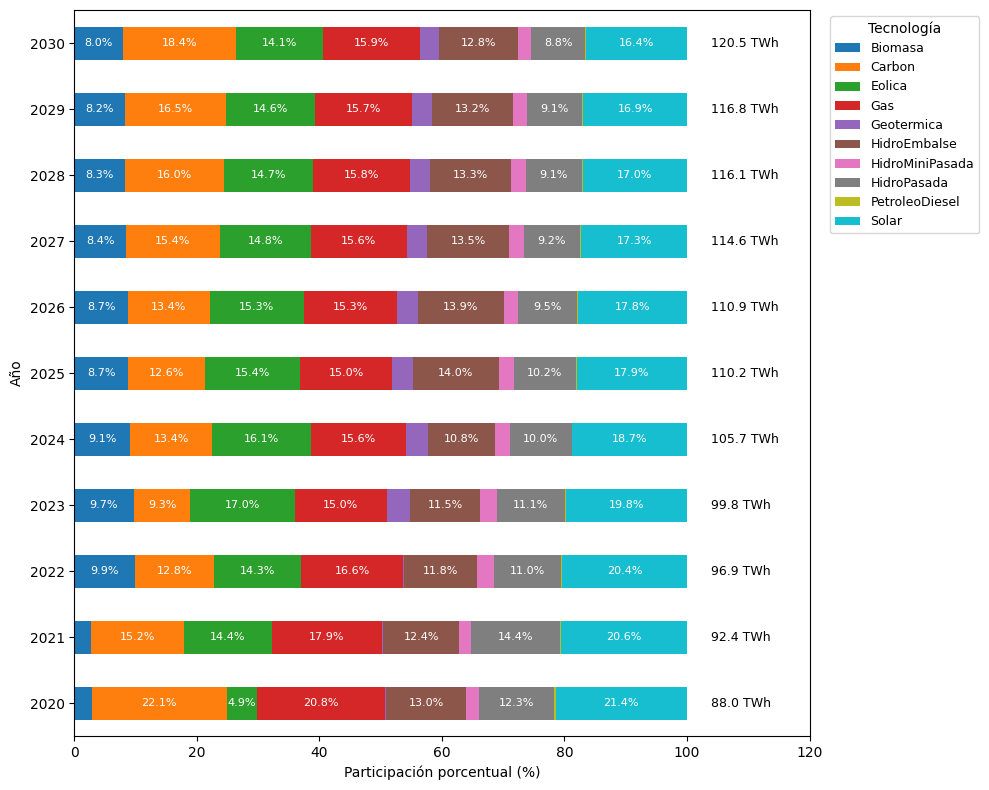
\includegraphics[width=1\linewidth]{figures/mprx0.0.png}
    \caption{Matriz energética horizonte 2020-2030 – Escenario 5 Distribución tecnológica por nivel de atención}
    \label{fig:produccion_matriz}
\end{figure}
La Figura \ref{fig:a.p.1}, por otro lado, compara los distintos niveles de atención para el año 2030 con el fin de entender cómo esta afecta el nivel productivo de las distintas tecnologías. Se observa que a medida que la atención aumenta también lo hacen las participaciones de las ERNC y a su vez se reducen las emisoras. El carbón se reduce significativamente desde un nivel de atención de 0 a 1 pasando de una participación de 18,4\% a 14,2\% a la vez que la eólica y la solar aumentan en 1,3 y 2,4 puntos porcentuales respectivamente.

\begin{figure}[H]
    \centering
    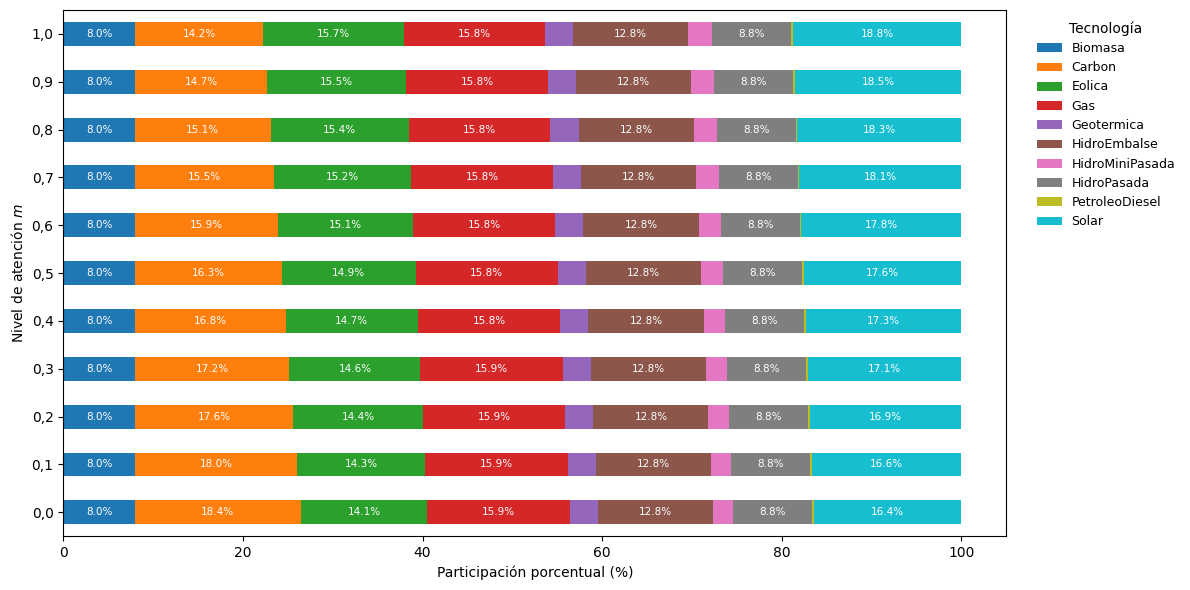
\includegraphics[width=1\linewidth]{figures/ngrafatencionporduccion.png}
    \caption{Matriz energética 2030 – Escenario 5 Distribución tecnológica por nivel de atención}
    \label{fig:a.p.1}
\end{figure}

El factor de emisión por tecnología representa cuánto contamina una tecnología en proporción a cuánta energía produce. El carbón y el petrodiésel tienen este valor en 0.91 tCO$_2$e/MWh y el gas en 0.65 tCO$_2$e/MWh (véase Anexo \ref{tab:epsilon}). Al multiplicar estos valores por su producción energética se obtiene la emisión de cada tecnología. Puede verse en la Figura \ref{fig:emisioneselec} cómo las emisiones se comportan a lo largo de los años para distintos niveles de atención: $m=0$, $m=0,5$, y $m=1$ y el promedio para cada nivel de $m$.  

\begin{figure}[H]
    \centering
    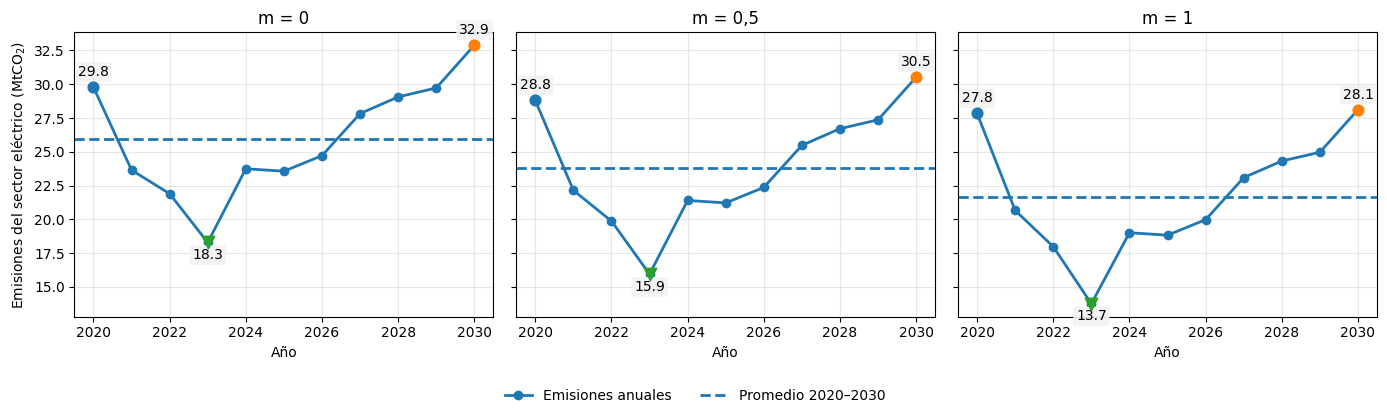
\includegraphics[width=1\linewidth]{figures/emisionesselectrico.png}
    \caption{Emisiones para el horizonte 2020-2030 en el sector eléctrico (Fuente: elaboración propia)}
    \label{fig:emisioneselec}
\end{figure}

Se puede notar como la tendencia de emisiones se mantiene con una estructura similar en los tres casos, sin embargo, el nivel de atención reduce el total de emisiones por año generando un promedio más bajo al aumentar la atención. El nivel de atención $m=1$ es el que más se aproxima a la meta de llegar a 95 MtCO$_2$e para el 2030, lo que proporcionalmente quiere decir que el sector eléctrico debiera tener un nivel de emisiones de 26,46  MtCO$_2$e, dada la proporción descrita en el capítulo \ref{c3}. Para los otros niveles de atención el nivel de emisiones se aleja aún más. 

En la Figura  \ref{fig:emisionesxtec} se presentan las emisiones por tecnología, se observa que dos tecnologías (gas y petrodiésel) mantienen niveles de emisión prácticamente rígidos frente a cambios en el nivel de atención del planificador. En cambio, el carbón es la única tecnología cuya trayectoria de emisiones varía de manera perceptible, lo que sugiere que esta opera con mayor holgura frente a cambios en el presupuesto de emisiones. 

\begin{figure}[H]
    \centering
    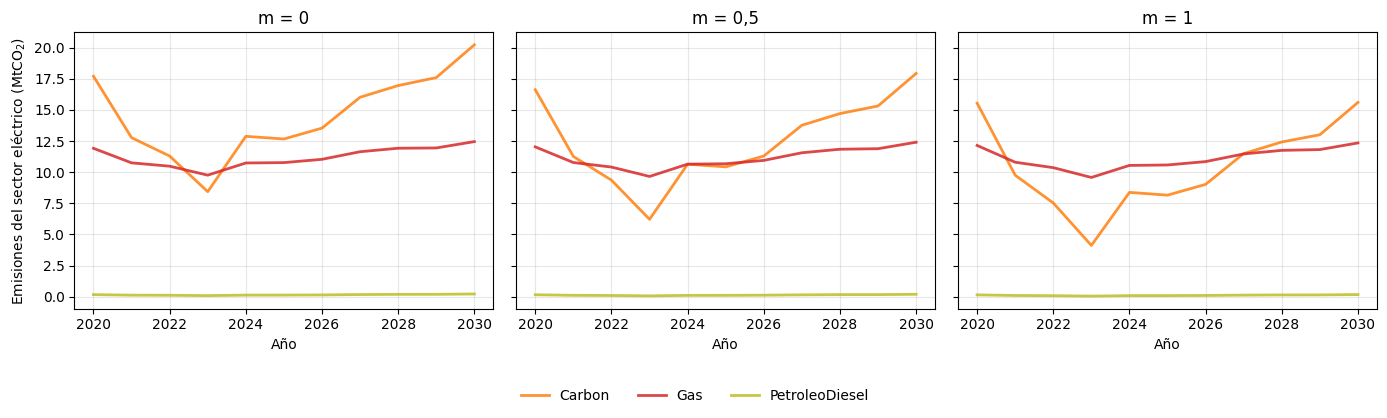
\includegraphics[width=1\linewidth]{figures/emisionxtec.png}
    \caption{Emisiones por tecnología para el horizonte 2020-2030 en el sector eléctrico (Fuente: elaboración propia)}
    \label{fig:emisionesxtec}
\end{figure}

Si bien la producción de las tecnologías emisoras presenta una tendencia creciente después de 2023, las fuentes no emisoras mantienen una participación mayoritaria en el mix, superando significativamente los niveles de generación de origen fósil. En la Figura \ref{fig:emisorasvslimpias} se comparan los niveles productivos de ambos tipos de energía para los niveles de atención $m=0$ y $m=1$, permitiendo visualizar la brecha entre la generación limpia y la emisora en función de la precisión de la señal.

\begin{figure}[H]
    \centering
    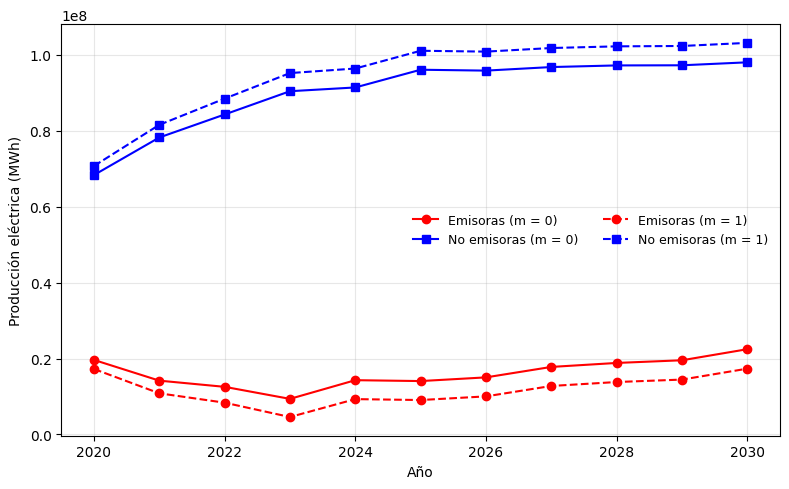
\includegraphics[width=0.75\linewidth]{figures/emislimp.png}
    \caption{Producción de tecnologías emisoras frente a limpias (Fuente: elaboración propia)}
    \label{fig:emisorasvslimpias}
\end{figure}
Las tecnologías ERNC crecen considerablemente desde el inicio del período hasta el final, mientras que las emisoras, si bien aumentan su producción, lo hacen en una escala mucho menor, obteniendo producciones muy similares en el 2030 que cuando comenzaron en 2020.




